\documentclass[12pt,a4paper]{report}

\usepackage[a4paper,margin=1in]{geometry}
\usepackage{graphicx}
\usepackage{titlesec}
\usepackage{setspace}
\usepackage{array}
\usepackage{longtable}
\usepackage{booktabs}
\usepackage{float}
\usepackage[hidelinks]{hyperref}
\usepackage{caption}
\usepackage{enumitem}
\usepackage{tikz}
\usetikzlibrary{shapes.geometric, arrows.meta, positioning}

\setstretch{1.3}

% Reduce spacing between bullet points
\setlist{nosep, topsep=0pt, partopsep=0pt, parsep=0pt, itemsep=2pt}

% Prevent chapters from starting on a new page
\titleclass{\chapter}{straight}
\titleformat{\chapter}[block]{\normalfont\LARGE\bfseries}{\thechapter.}{1em}{}
\titlespacing*{\chapter}{0pt}{3.5ex plus 1ex minus .2ex}{2.3ex plus .2ex}

\begin{document}

%------------------------------------------------
% TITLE PAGE
%------------------------------------------------

\begin{titlepage}
    \centering
    
    \vspace*{1cm}
    
    {\Huge \textbf{Schlopify}}\\[0.5cm]
    
    {\Large A Kubernetes-Based Multi-Tenant E-Commerce Platform}\\[1.5cm]
    
    \textbf{Final Project Report}\\[0.3cm]
    submitted in partial fulfillment of the requirements for the course\\[0.2cm]
    
    {\Large \textbf{CSE 816: Software Production Engineering}}\\[1.5cm]
    
    \vfill
    
    \textbf{Submitted By:}\\[0.5cm]
    
    \begin{tabular}{ll}
        Aniket Kumar & (MT2025019) \\
        Shreyas Gangurde & (MT2025117) \\
    \end{tabular}
    
    \vspace{1.5cm}
    
    \textbf{Department of Computer Science and Engineering}\\
    International Institute of Information Technology Bangalore\\
    Bengaluru, Karnataka, India
    
    \vfill
    
    \textbf{Academic Year: 2025--2026}
    
\end{titlepage}

\tableofcontents
\newpage


%------------------------------------------------
% ABSTRACT
%------------------------------------------------

\chapter*{Abstract}
\addcontentsline{toc}{chapter}{Abstract}

Modern cloud-native applications require scalable and automated deployment infrastructures capable of efficiently managing multiple tenants and services. Traditional deployment approaches often struggle to provide the scalability, flexibility, and isolation required by modern Software-as-a-Service (SaaS) platforms. To address these challenges, this project presents \textbf{Schlopify}, a Kubernetes-based multi-tenant e-commerce platform designed to dynamically provision isolated storefronts for users.

The platform utilizes Docker for containerization and Kubernetes for orchestration to deploy and manage multiple microservices, including authentication services, frontend applications, APIs, PostgreSQL databases, and PostgREST instances. A key feature of the system is the dynamic tenant provisioning mechanism implemented using Golang. Whenever a new shop is created, the backend automatically interacts with the Kubernetes API to generate dedicated namespaces, deploy databases, configure ingress routing, and provision tenant-specific services.

The project also integrates Horizontal Pod Autoscaling (HPA) to improve scalability and resource utilization. Kubernetes deployments and ingress configurations ensure reliable service accessibility and efficient workload management within local Kubernetes environments such as Minikube and Kind.

The project also incorporates a CI/CD pipeline using Jenkins with GitHub webhook-based triggers, Ansible for configuration management and deployment automation, and the ELK Stack (Elasticsearch, Logstash, Kibana) for centralized logging and monitoring. Although Vault-based secret management is not fully integrated in the current implementation, the system architecture has been designed to support this feature in future enhancements.

Overall, Schlopify demonstrates the practical implementation of DevOps methodologies, microservices architecture, and Kubernetes-based orchestration for building scalable and isolated SaaS platforms.

\newpage












%------------------------------------------------
% INTRODUCTION
%------------------------------------------------

\chapter{Introduction}

Modern cloud-native applications require scalable and automated infrastructures capable of handling multiple users and services efficiently. Traditional deployment methods often struggle with scalability, resource management, and tenant isolation, making them less suitable for modern Software-as-a-Service (SaaS) platforms. DevOps practices combined with container orchestration technologies have become essential for building reliable and scalable applications.

This project, titled \textbf{Schlopify}, is a Kubernetes-based multi-tenant e-commerce platform designed to dynamically provision isolated storefront environments for users. The platform uses Docker for containerization and Kubernetes for orchestration and deployment of various microservices, including frontend applications, APIs, authentication services, and databases.

A major feature of the platform is its dynamic tenant provisioning system implemented using Golang. Whenever a new tenant registers, the backend automatically creates dedicated Kubernetes namespaces, deploys databases and services, configures ingress routing, and provisions tenant-specific resources. The project also incorporates Horizontal Pod Autoscaling (HPA) to improve scalability and resource utilization.

Overall, Schlopify demonstrates the practical implementation of DevOps methodologies, microservices architecture, and Kubernetes-based orchestration for building scalable SaaS applications.

\newpage











%------------------------------------------------
% PROBLEM STATEMENT
%------------------------------------------------

\chapter{Problem Statement}

Modern e-commerce platforms and SaaS applications require scalable infrastructures capable of supporting multiple tenants simultaneously while maintaining isolation, reliability, and efficient resource utilization. Traditional deployment approaches often rely on manually configured servers and monolithic architectures, which make scaling, maintenance, and tenant management difficult.

Managing separate infrastructures for each tenant increases operational complexity and resource overhead. Additionally, deploying new tenant environments manually is time-consuming and error-prone. As the number of users grows, maintaining high availability, scalability, and efficient deployment workflows becomes increasingly challenging.

Another major challenge is ensuring proper tenant isolation while still utilizing shared infrastructure resources effectively. Without automation and orchestration, provisioning databases, APIs, frontend services, networking configurations, and scaling policies for each tenant becomes difficult to manage.

The objective of this project is to design and implement an automated cloud-native platform that dynamically provisions isolated e-commerce storefronts for different tenants using Kubernetes orchestration and containerized microservices. The platform aims to simplify deployment, improve scalability, and automate tenant management using modern DevOps methodologies.

\newpage






%------------------------------------------------
% OBJECTIVES
%------------------------------------------------

\chapter{Objectives}

The primary objective of this project is to design and implement a scalable multi-tenant e-commerce platform using modern DevOps and cloud-native technologies. The project focuses on automating deployment workflows, improving scalability, and ensuring tenant isolation using Kubernetes orchestration.

The major objectives of the project are as follows:

\begin{itemize}

    \item Develop a multi-tenant e-commerce platform capable of dynamically provisioning isolated storefront environments for users.

    \item Utilize Docker for containerizing application services and ensuring portability across deployment environments.

    \item Deploy and manage microservices using Kubernetes orchestration.

    \item Automate tenant provisioning using Kubernetes APIs and Golang-based backend services.

    \item Implement dedicated namespaces and isolated resources for each tenant to ensure security and scalability.

    \item Configure ingress routing and networking for tenant-specific service accessibility.

    \item Implement Horizontal Pod Autoscaling (HPA) for dynamic scaling and efficient resource utilization.

    \item Follow DevOps methodologies for infrastructure automation and cloud-native application deployment.

    \item Integrate Jenkins CI/CD pipelines with GitHub webhook triggers for automated build and deployment workflows.

    \item Implement Ansible-based configuration management for repeatable infrastructure provisioning.

    \item Deploy the ELK Stack for centralized logging and monitoring of platform services.

\end{itemize}












\newpage
%------------------------------------------------
% EXISTING SYSTEM VS PROPOSED SYSTEM
%------------------------------------------------

\chapter{Existing System vs Proposed System}

\section{Existing System}

Traditional e-commerce platforms are generally deployed using monolithic architectures where all application components are tightly coupled and hosted on shared infrastructure. Such systems often require manual deployment, configuration, and scaling processes, which increase operational complexity and maintenance overhead.

In conventional deployment models, onboarding a new tenant or customer may require manual database setup, service configuration, and infrastructure provisioning. These approaches are time-consuming and difficult to scale efficiently. Additionally, resource sharing without proper isolation can create security and performance concerns among tenants.

Most traditional systems also lack automated orchestration and dynamic scaling capabilities, resulting in inefficient resource utilization and reduced flexibility during varying workloads.

\section{Proposed System}

The proposed system, \textbf{Schlopify}, addresses these limitations by implementing a cloud-native, Kubernetes-based multi-tenant architecture. The platform dynamically provisions isolated storefront environments for tenants using containerized microservices and Kubernetes orchestration.

Each tenant is assigned dedicated namespaces, databases, APIs, and frontend services, ensuring strong isolation and scalability. Docker is used for containerization, while Kubernetes manages deployment, networking, scaling, and orchestration of services.

The platform also includes automated tenant provisioning implemented using Golang and Kubernetes APIs. Whenever a new tenant registers, the backend automatically creates the required infrastructure components, configures ingress routing, and deploys tenant-specific services.

Additionally, Horizontal Pod Autoscaling (HPA) improves scalability by dynamically adjusting application resources based on workload demands. The platform also integrates Jenkins for CI/CD automation with GitHub webhook triggers, Ansible for configuration management, and the ELK Stack for centralized logging and monitoring.














\newpage

%------------------------------------------------
% SYSTEM ARCHITECTURE
%------------------------------------------------

\chapter{System Architecture}

The architecture of Schlopify follows a cloud-native microservices approach designed to support scalability, tenant isolation, and automated infrastructure provisioning. The platform is built using Docker and Kubernetes, where each major component operates as an independent containerized service within the Kubernetes cluster.

The system consists of two primary layers:

\begin{enumerate}

    \item \textbf{Control Plane}
    
    The control plane is responsible for managing the core functionality of the platform. It includes:
    
    \begin{itemize}
        \item Authentication Service
        \item Platform Frontend
        \item Platform API
        \item Tenant Provisioning Logic
    \end{itemize}
    
    These services handle user authentication, tenant registration, infrastructure provisioning, and overall platform management.

    \item \textbf{Tenant Infrastructure}
    
    Whenever a new tenant registers on the platform, the backend dynamically provisions a dedicated environment inside Kubernetes. Each tenant receives:
    
    \begin{itemize}
        \item Separate Kubernetes Namespace
        \item Dedicated PostgreSQL Database
        \item PostgREST API Service
        \item Isolated Frontend Storefront
        \item Ingress Configuration for Routing
    \end{itemize}
    
    This architecture ensures proper isolation, scalability, and simplified management of tenant resources.

\end{enumerate}

Docker is used to package all application components into portable containers, while Kubernetes handles deployment, orchestration, networking, and scaling of services. Ingress resources are configured to provide tenant-specific routing using local DNS resolution with \texttt{nip.io}.

The platform also incorporates Horizontal Pod Autoscaling (HPA) for dynamically scaling PostgREST services based on workload requirements. Automated provisioning is implemented using Golang, where the backend interacts directly with Kubernetes APIs to create namespaces, deployments, services, and scaling policies.

\begin{figure}[H]
    \centering
    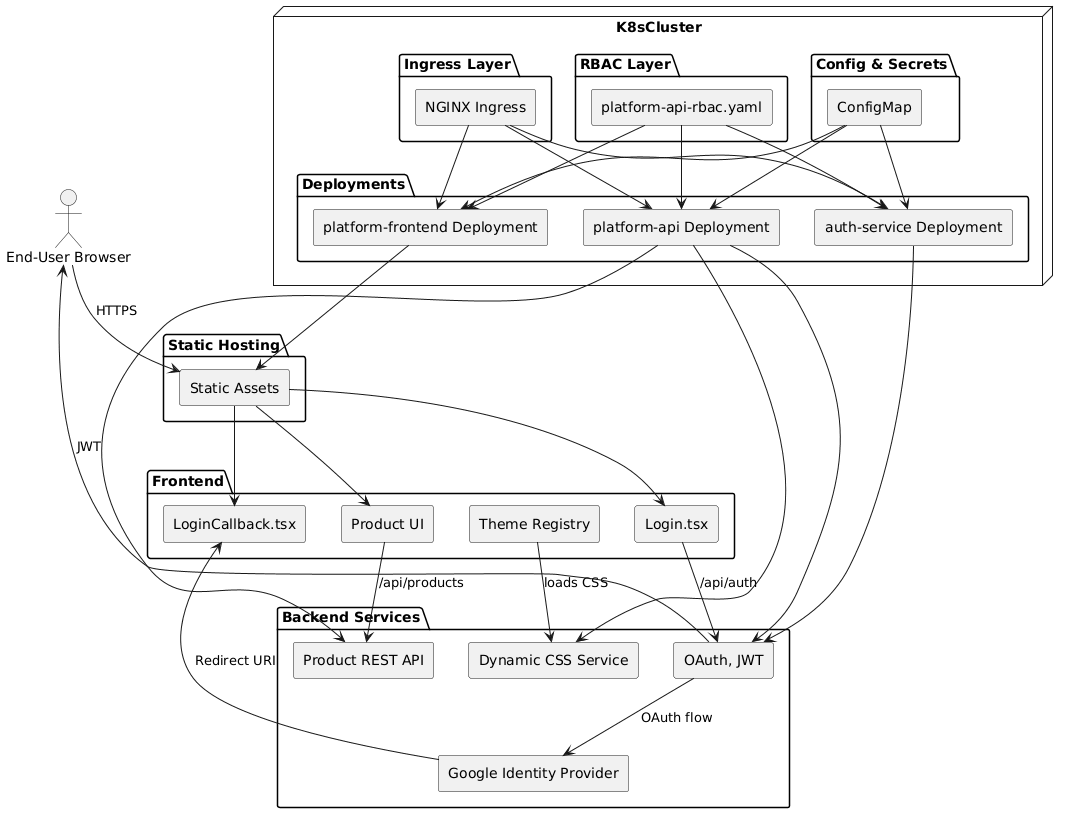
\includegraphics[width=\textwidth]{images/architectural diagram.png}
    \caption{System Architecture Diagram}
\end{figure}















\newpage
%------------------------------------------------
% TECHNOLOGY STACK
%------------------------------------------------

\chapter{Technology Stack}

The Schlopify platform utilizes multiple cloud-native and DevOps technologies to implement scalable deployment, orchestration, tenant provisioning, and microservices management. The following technologies were used during the development and deployment of the project.

\section{Programming Languages}

\begin{itemize}

    \item \textbf{Golang} \\
    Used for implementing backend APIs, tenant provisioning logic, and Kubernetes API interactions.

    \item \textbf{JavaScript / TypeScript} \\
    Used for developing frontend applications and platform interfaces.

\end{itemize}

\section{Containerization}

\begin{itemize}

    \item \textbf{Docker} \\
    Docker was used to containerize all major application components, including frontend services, backend APIs, authentication services, and database-related components. Containerization ensured portability and simplified deployment across Kubernetes environments.

\end{itemize}

\section{Container Orchestration}

\begin{itemize}

    \item \textbf{Kubernetes} \\
    Kubernetes was used as the primary orchestration platform for managing deployments, namespaces, services, ingress resources, RBAC configurations, and scaling operations.

    \item \textbf{Minikube and Kind} \\
    Local Kubernetes environments such as Minikube and Kind were used for development, testing, and deployment purposes.

\end{itemize}

\section{Database Technologies}

\begin{itemize}

    \item \textbf{PostgreSQL} \\
    PostgreSQL databases were dynamically provisioned for each tenant to ensure data isolation and reliable storage management.

    \item \textbf{PostgREST} \\
    PostgREST was used to expose PostgreSQL databases as RESTful APIs for tenant applications.

\end{itemize}

\section{Networking and Routing}

\begin{itemize}

    \item \textbf{Kubernetes Ingress} \\
    Ingress resources were configured to enable tenant-specific routing and service accessibility.

    \item \textbf{nip.io} \\
    Used for local DNS-based routing during development and testing.

\end{itemize}

\section{Scaling and Resource Management}

\begin{itemize}

    \item \textbf{Horizontal Pod Autoscaler (HPA)} \\
    HPA was implemented to dynamically scale PostgREST services based on workload requirements and resource utilization.

\end{itemize}

\section{CI/CD and Automation}

\begin{itemize}

    \item \textbf{Jenkins} \\
    Jenkins is used for CI/CD pipeline automation, handling source code builds, Docker image generation, and Kubernetes deployment rollouts.

    \item \textbf{GitHub Webhooks} \\
    GitHub push webhooks are configured to automatically trigger Jenkins pipelines whenever changes are pushed to the repository.

\end{itemize}

\section{Configuration Management}

\begin{itemize}

    \item \textbf{Ansible} \\
    Ansible playbooks are used for infrastructure automation and configuration management, enabling repeatable provisioning of platform components.

\end{itemize}

\section{Monitoring and Logging}

\begin{itemize}

    \item \textbf{ELK Stack (Elasticsearch, Logstash, Kibana)} \\
    The ELK Stack provides centralized logging and monitoring. Logstash collects logs from platform services, Elasticsearch indexes them, and Kibana provides dashboards for visualization and analysis.

\end{itemize}










\newpage
%------------------------------------------------
% DEPLOYMENT WORKFLOW
%------------------------------------------------

\chapter{Deployment Workflow}

The deployment workflow of Schlopify is designed to automate the provisioning and management of tenant-specific infrastructures using Kubernetes and containerized microservices. The overall deployment process is divided into two major stages: control plane deployment and dynamic tenant provisioning.

\section{Control Plane Deployment}

The control plane contains the core services responsible for managing the platform and handling tenant provisioning operations. Deployment of the control plane is performed locally using custom deployment scripts.

The deployment workflow is as follows:

\begin{enumerate}

    \item Execute the deployment script using \texttt{deploy.sh}.

    \item Build Docker images for all platform services including:
    \begin{itemize}
        \item Platform Frontend
        \item Platform API
        \item Authentication Service
        \item Tenant Frontend Services
    \end{itemize}

    \item Load the generated Docker images into the Kubernetes cluster.

    \item Apply Kubernetes manifests including:
    \begin{itemize}
        \item Namespaces
        \item Deployments
        \item Services
        \item RBAC Policies
        \item Ingress Resources
    \end{itemize}

    \item Initialize the platform services and expose them through ingress routing.

\end{enumerate}

After successful deployment, the platform becomes ready for tenant provisioning and management.

\section{Dynamic Tenant Provisioning}

One of the major features of Schlopify is its ability to dynamically provision isolated infrastructures for tenants using Kubernetes APIs.

Whenever a new tenant registers on the platform, the following workflow is executed automatically:

\begin{enumerate}

    \item User submits shop registration details through the platform frontend.

    \item Platform API receives the request and invokes the provisioning logic implemented in Golang.

    \item A dedicated Kubernetes namespace is created for the tenant.

    \item PostgreSQL database services are deployed and initialized.

    \item PostgREST API services are provisioned.

    \item Horizontal Pod Autoscaling (HPA) configurations are applied.

    \item Frontend storefront services are deployed for the tenant.

    \item Kubernetes ingress resources are configured for tenant-specific routing.

    \item The tenant storefront becomes accessible through the assigned domain.

\end{enumerate}

This automated provisioning workflow simplifies infrastructure management while ensuring scalability, isolation, and efficient resource utilization.

\begin{figure}[H]
    \centering
    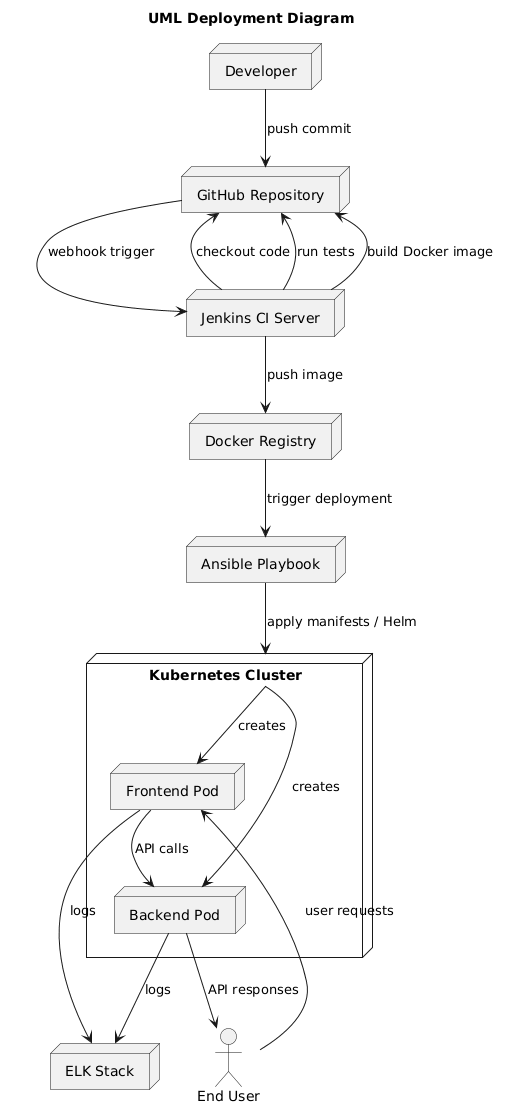
\includegraphics[width=0.6\textwidth]{images/deply flow.png}
    \caption{Deployment Workflow Diagram}
\end{figure}

\section{Deployment Script (\texttt{deploy.sh})}

The platform control plane is deployed using a single shell script, \texttt{deploy.sh}, which automates the entire build-load-deploy pipeline. The script accepts the cluster type (Minikube or Kind) as a parameter and performs the following stages:

\begin{enumerate}
    \item \textbf{Image Build} — Builds Docker images for the shop frontend, platform frontend, auth server, and platform API.
    \item \textbf{Cluster Load} — Loads the built images into the local Kubernetes cluster (Minikube or Kind).
    \item \textbf{Auth System Setup} — Applies namespace, deployment, and ingress manifests for the authentication service.
    \item \textbf{Platform Setup} — Creates the platform namespace, applies RBAC policies, and deploys the platform API, frontend, and ingress.
    \item \textbf{Readiness Wait} — Waits for the platform API and auth server deployments to become available before declaring success.
\end{enumerate}

The following diagram illustrates the execution flow of the deployment script:

\begin{figure}[H]
\centering
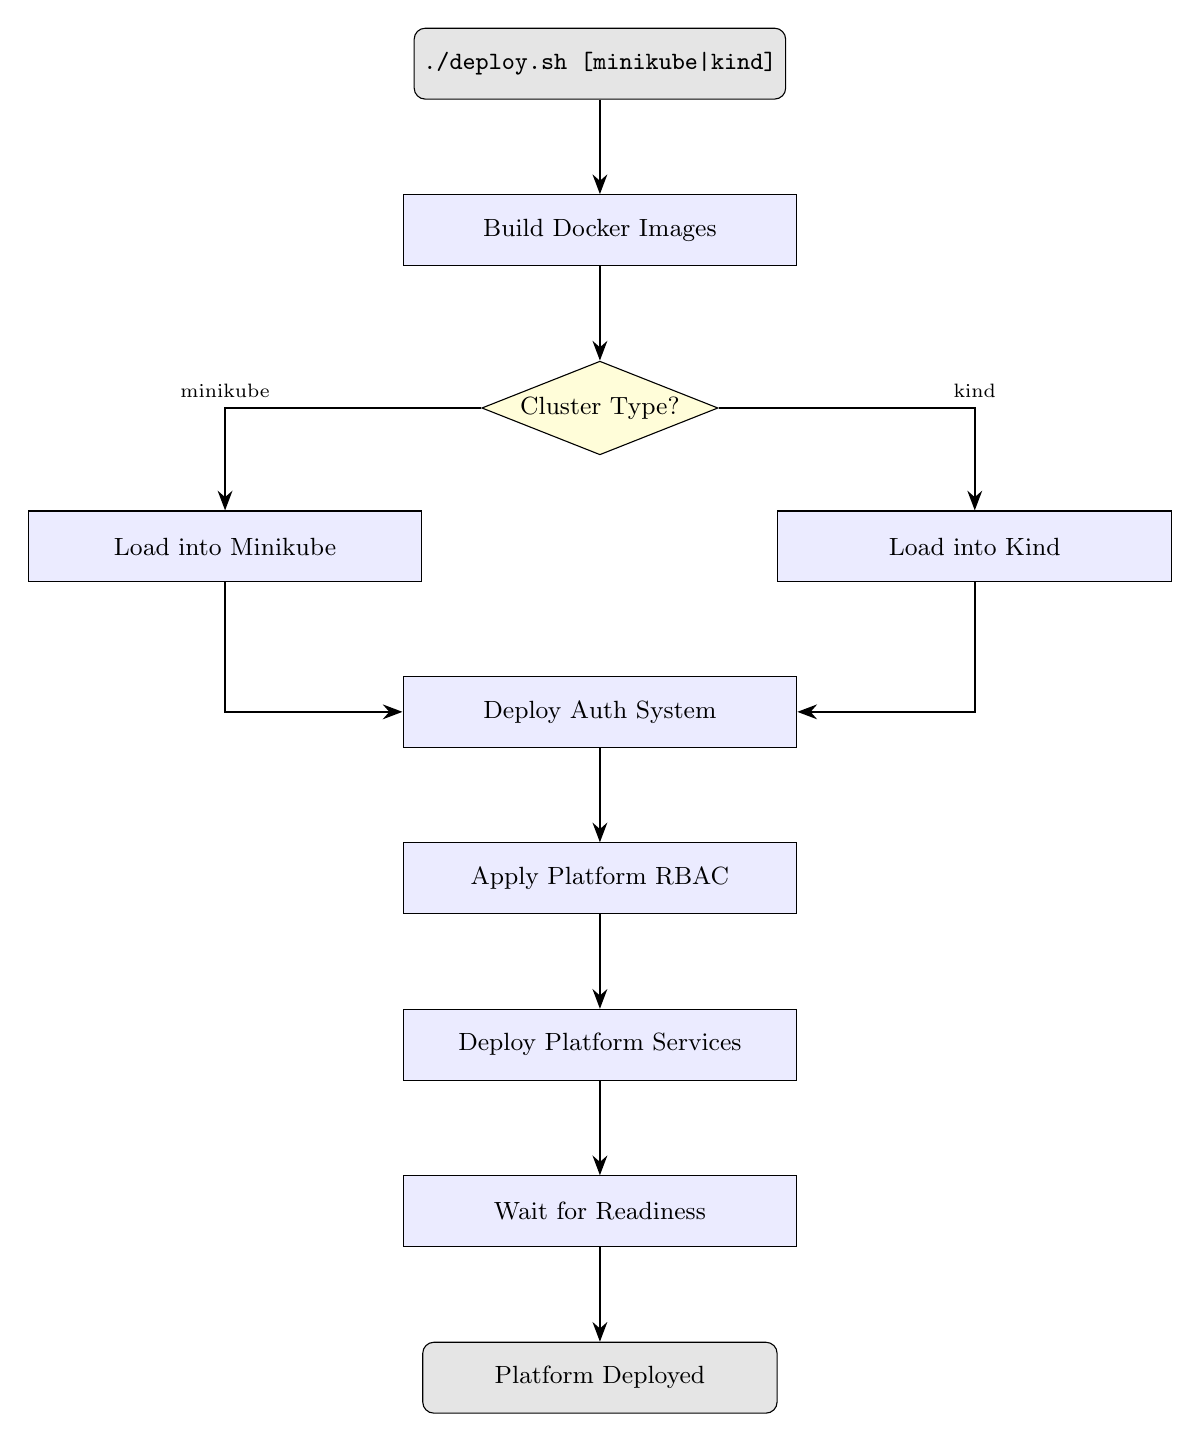
\begin{tikzpicture}[
    node distance=1.2cm,
    startstop/.style={rectangle, rounded corners, minimum width=4.5cm, minimum height=0.9cm, text centered, draw=black, fill=black!10, font=\small},
    process/.style={rectangle, minimum width=5cm, minimum height=0.9cm, text centered, draw=black, fill=blue!8, font=\small},
    decision/.style={diamond, aspect=2.5, minimum width=3cm, text centered, draw=black, fill=yellow!15, font=\small, inner sep=1pt},
    arrow/.style={-{Stealth[length=2.5mm]}, thick}
]

\node (start) [startstop] {\texttt{./deploy.sh [minikube|kind]}};
\node (build) [process, below=of start] {Build Docker Images};
\node (decide) [decision, below=of build] {Cluster Type?};
\node (mini) [process, below left=1cm and 1.5cm of decide] {Load into Minikube};
\node (kind) [process, below right=1cm and 1.5cm of decide] {Load into Kind};
\node (auth) [process, below=2.8cm of decide] {Deploy Auth System};
\node (rbac) [process, below=of auth] {Apply Platform RBAC};
\node (plat) [process, below=of rbac] {Deploy Platform Services};
\node (wait) [process, below=of plat] {Wait for Readiness};
\node (done) [startstop, below=of wait] {Platform Deployed};

\draw [arrow] (start) -- (build);
\draw [arrow] (build) -- (decide);
\draw [arrow] (decide) -| node[above, font=\scriptsize] {minikube} (mini);
\draw [arrow] (decide) -| node[above, font=\scriptsize] {kind} (kind);
\draw [arrow] (mini) |- (auth);
\draw [arrow] (kind) |- (auth);
\draw [arrow] (auth) -- (rbac);
\draw [arrow] (rbac) -- (plat);
\draw [arrow] (plat) -- (wait);
\draw [arrow] (wait) -- (done);

\end{tikzpicture}
\caption{Deployment Script (\texttt{deploy.sh}) Execution Flow}
\end{figure}








\newpage
%------------------------------------------------
% MULTI-TENANT ARCHITECTURE
%------------------------------------------------

\chapter{Multi-Tenant Architecture}

Schlopify is designed as a multi-tenant e-commerce platform where multiple independent storefronts can operate simultaneously on shared Kubernetes infrastructure while maintaining logical isolation between tenants. The architecture focuses on scalability, automation, and efficient resource utilization.

\section{Tenant Isolation}

Each tenant is provisioned with a dedicated Kubernetes namespace. This namespace contains all resources associated with the tenant, including:

\begin{itemize}

    \item PostgreSQL Database
    \item PostgREST API Services
    \item Frontend Storefront
    \item Kubernetes Services
    \item Ingress Configurations

\end{itemize}

Using separate namespaces ensures strong logical isolation between tenants and simplifies resource management, monitoring, and deployment operations.

\section{Dynamic Provisioning}

Tenant environments are dynamically created using Kubernetes APIs through backend provisioning logic implemented in Golang. Whenever a new tenant registers on the platform, the system automatically provisions all required infrastructure resources without manual intervention.

The provisioning process includes:

\begin{itemize}

    \item Namespace creation
    \item Database deployment and initialization
    \item API service deployment
    \item Frontend deployment
    \item Ingress configuration
    \item HPA configuration

\end{itemize}

This automated approach significantly reduces operational complexity and improves deployment efficiency.

\section{Microservices-Based Design}

The platform follows a microservices architecture where each major component operates independently as a containerized service. This modular design improves maintainability, scalability, and fault isolation.

The architecture consists of:

\begin{itemize}

    \item Authentication Services
    \item Platform APIs
    \item Frontend Applications
    \item Tenant APIs
    \item Database Services

\end{itemize}

Each service can be independently deployed, updated, and scaled according to workload requirements.

\section{Scalability and Resource Management}

Kubernetes orchestration enables efficient management of workloads and infrastructure resources. Horizontal Pod Autoscaling (HPA) is used to dynamically scale PostgREST services based on application load and resource utilization.

The platform architecture is also designed to support future integrations such as centralized monitoring, CI/CD pipelines, and advanced security management tools.














\newpage
%------------------------------------------------
% DOCKERIZATION AND CONTAINER MANAGEMENT
%------------------------------------------------

\chapter{Dockerization and Container Management}

Containerization plays a major role in the deployment architecture of Schlopify. Docker was used to package all application components into lightweight and portable containers, enabling consistent execution across different Kubernetes environments.

\section{Use of Docker}

Each major service in the platform was containerized using separate Docker images. This approach simplified deployment, dependency management, and scalability of the system.

The following services were containerized:

\begin{itemize}

    \item Platform Frontend
    \item Platform API
    \item Authentication Service
    \item Tenant Storefront Frontend
    \item PostgREST API Services

\end{itemize}

Docker images were locally built during deployment and loaded into Kubernetes clusters such as Minikube and Kind.

\section{Benefits of Containerization}

The use of Docker provided several advantages during development and deployment:

\begin{itemize}

    \item Consistent execution environments across systems
    \item Simplified dependency management
    \item Faster deployment and scaling
    \item Improved portability and maintainability
    \item Isolation between services
    \item Easier integration with Kubernetes orchestration

\end{itemize}

\section{Image Build and Deployment Process}

Docker images are generated during the deployment process and pushed to Docker Hub as part of the Jenkins CI/CD pipeline. The deployment workflow performs the following operations:

\begin{enumerate}

    \item Build Docker images for all services
    \item Tag container images appropriately
    \item Push images to Docker Hub for centralized storage
    \item Pull and load images into the Kubernetes cluster
    \item Deploy services using Kubernetes manifests

\end{enumerate}

This automated workflow reduces manual deployment effort and ensures consistency during infrastructure provisioning.

\section{Future Enhancements}

Future improvements can include:

\begin{itemize}

    \item Image vulnerability scanning
    \item Multi-stage Docker builds for optimization
    \item Container monitoring and logging systems

\end{itemize}















\newpage
%------------------------------------------------
% KUBERNETES ORCHESTRATION
%------------------------------------------------

\chapter{Kubernetes Orchestration}

Kubernetes serves as the core orchestration platform for Schlopify and is responsible for managing deployments, networking, scaling, and tenant isolation across the entire system. The project utilizes Kubernetes to automate infrastructure management and simplify deployment operations for containerized microservices.

\section{Deployment Management}

Kubernetes Deployments are used to manage application services such as frontend applications, APIs, authentication services, PostgreSQL databases, and PostgREST instances. Deployments ensure that the required number of pods remain active and automatically recover failed containers when necessary.

The orchestration platform enables:

\begin{itemize}

    \item Automated deployment of services
    \item Pod management and recovery
    \item Rolling updates for applications
    \item Resource allocation and scheduling
    \item Simplified infrastructure management

\end{itemize}

\section{Namespaces and Tenant Isolation}

A dedicated Kubernetes namespace is dynamically created for each tenant. These namespaces isolate tenant-specific resources and simplify infrastructure management.

Each namespace contains:

\begin{itemize}

    \item Database deployments
    \item API services
    \item Frontend services
    \item Networking resources
    \item Scaling configurations

\end{itemize}

Namespace-based isolation improves scalability, maintainability, and security of the platform.

\section{Services and Networking}

Kubernetes Services are used to expose internal application components and enable communication between microservices. Ingress resources are configured to route incoming traffic to tenant-specific applications.

The platform uses \texttt{nip.io} for local DNS-based routing during development and testing.

\section{RBAC and Resource Management}

Role-Based Access Control (RBAC) policies are implemented to manage permissions and restrict access to Kubernetes resources. RBAC improves operational security and ensures controlled interactions between services and infrastructure components.

\section{Horizontal Pod Autoscaling}

Horizontal Pod Autoscaling (HPA) is implemented to dynamically scale PostgREST services based on workload requirements. This improves resource utilization and enables the platform to efficiently handle varying traffic loads.

\section{Local Kubernetes Environments}

The project supports local Kubernetes environments such as:

\begin{itemize}

    \item Minikube
    \item Kind (Kubernetes in Docker)

\end{itemize}

These environments were used for development, testing, and deployment of the platform.

\begin{figure}[H]
    \centering
    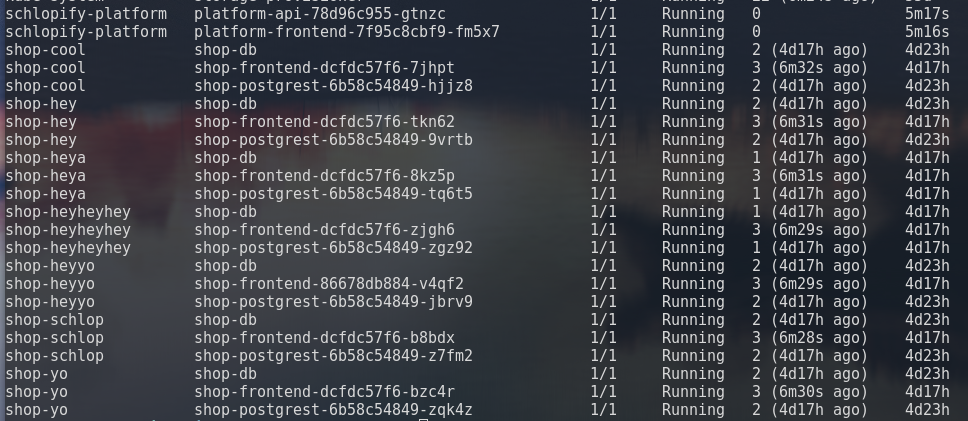
\includegraphics[width=\textwidth]{images/pods-list.png}
    \caption{Kubernetes Pods and Services}
\end{figure}














\newpage
%------------------------------------------------
% DYNAMIC TENANT PROVISIONING
%------------------------------------------------

\chapter{Dynamic Tenant Provisioning}

One of the most important features of Schlopify is its ability to dynamically provision complete tenant-specific infrastructures using Kubernetes APIs. The provisioning system automates the deployment of isolated environments for each tenant without requiring manual configuration or infrastructure setup.

\section{Provisioning Workflow}

Whenever a new tenant registers on the platform, the backend provisioning service automatically performs a sequence of infrastructure operations. These operations are implemented using Golang and Kubernetes client libraries.

The provisioning workflow includes the following steps:

\begin{enumerate}

    \item Receive tenant registration request from the frontend interface.

    \item Generate a unique Kubernetes namespace for the tenant.

    \item Deploy PostgreSQL database services within the namespace.

    \item Initialize required database schemas and configurations.

    \item Deploy PostgREST API services.

    \item Configure Horizontal Pod Autoscaler (HPA) policies.

    \item Deploy tenant-specific storefront frontend services.

    \item Configure Kubernetes ingress resources for external routing.

    \item Expose the tenant storefront through a dedicated domain.

\end{enumerate}

\section{Advantages of Dynamic Provisioning}

The automated provisioning mechanism provides several operational and architectural advantages:

\begin{itemize}

    \item Eliminates manual infrastructure configuration
    \item Reduces deployment time
    \item Improves scalability and consistency
    \item Simplifies tenant onboarding
    \item Ensures strong resource isolation
    \item Enables efficient infrastructure management

\end{itemize}

\section{Kubernetes API Integration}

The provisioning logic directly interacts with Kubernetes APIs to dynamically create and manage infrastructure resources. This allows the platform to automatically deploy namespaces, services, deployments, ingress resources, and scaling configurations during runtime.

Using Kubernetes APIs programmatically enables Schlopify to function as a self-managing cloud-native platform capable of handling tenant lifecycle operations efficiently.

\section{Scalability Considerations}

The architecture is designed to support multiple tenants simultaneously while maintaining isolation between workloads. Kubernetes orchestration and HPA integration ensure that services can scale dynamically based on demand and resource utilization.

\begin{figure}[H]
    \centering
    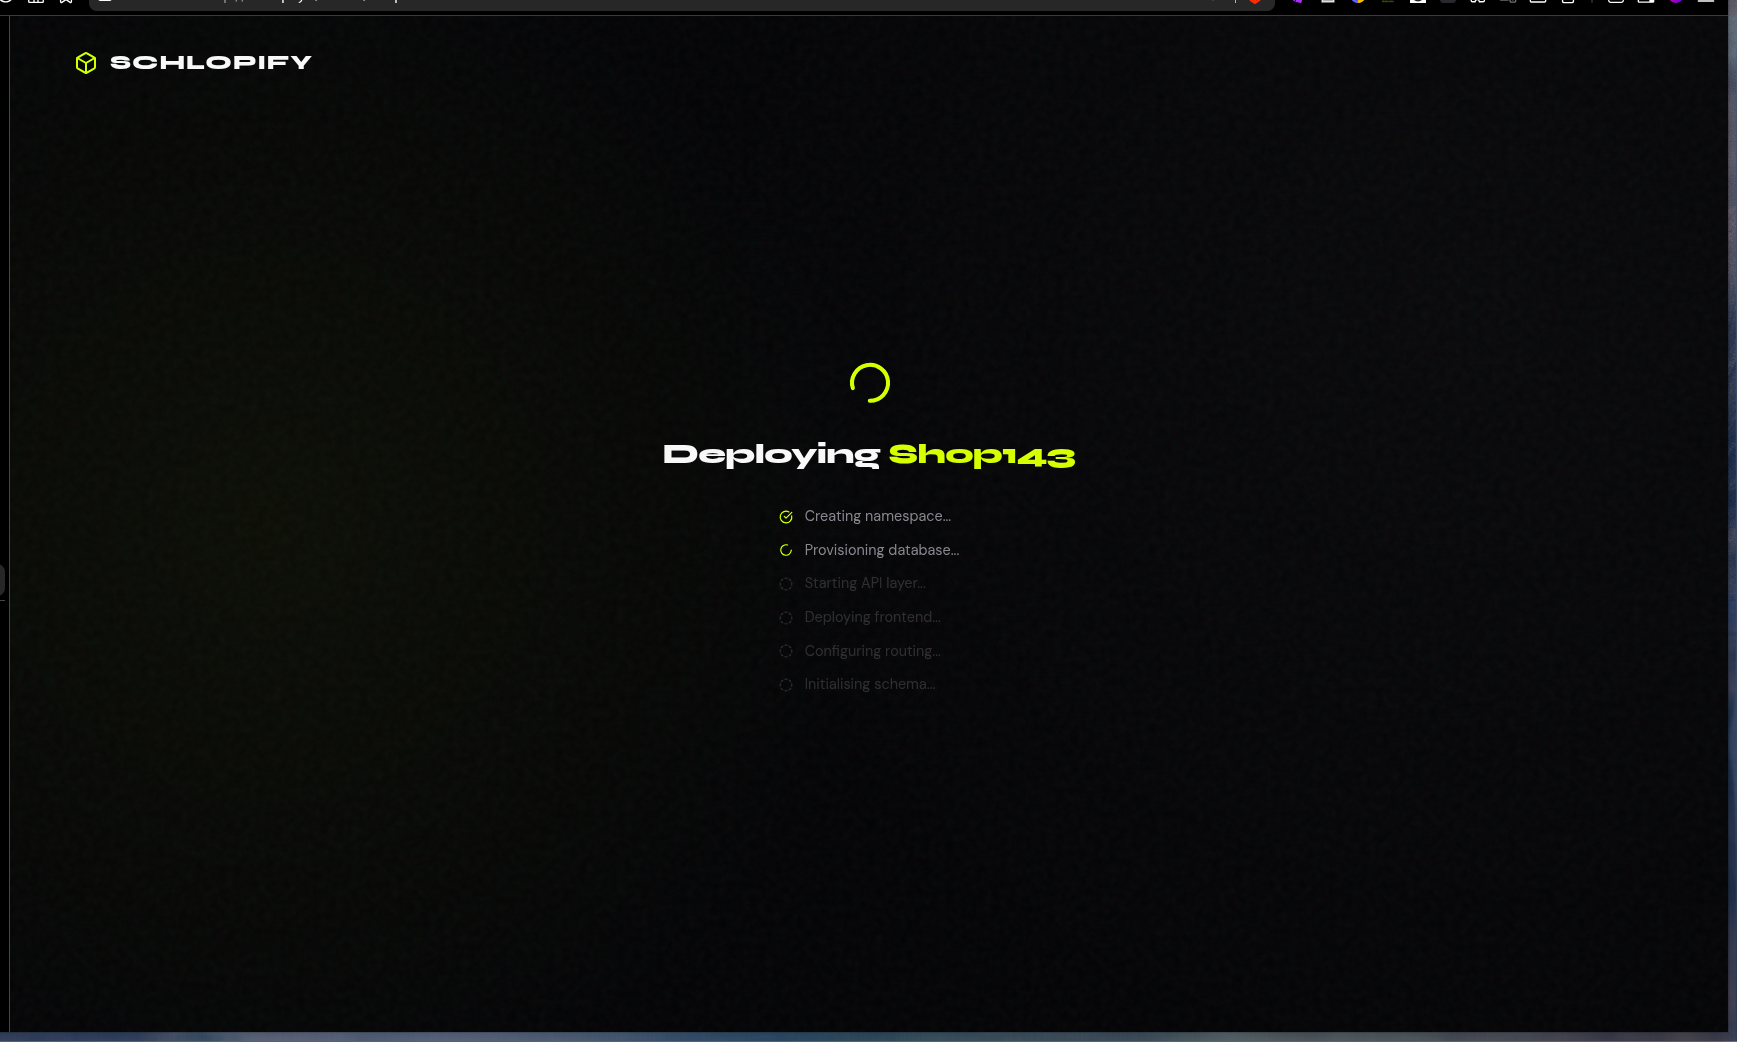
\includegraphics[width=\textwidth]{images/ui-2.png}
    \caption{Dynamic Tenant Provisioning in Progress}
\end{figure}


















\newpage

%------------------------------------------------
% HORIZONTAL POD AUTOSCALING
%------------------------------------------------

\chapter{Horizontal Pod Autoscaling}

Scalability is an important requirement for modern cloud-native applications. To efficiently handle varying workloads and optimize resource utilization, Schlopify integrates Kubernetes Horizontal Pod Autoscaling (HPA) for selected services within the platform.

\section{Overview of HPA}

Horizontal Pod Autoscaling is a Kubernetes feature that automatically adjusts the number of running pods for a deployment based on resource usage or workload metrics. This helps maintain application performance during high traffic conditions while avoiding unnecessary resource consumption during low workloads.

In Schlopify, HPA is primarily configured for PostgREST API services deployed for tenant environments.

\section{Implementation}

The HPA configuration is dynamically applied during tenant provisioning through backend logic implemented in Golang. When a new tenant environment is created, the provisioning system automatically deploys scaling policies for the corresponding PostgREST services.

The autoscaling mechanism monitors workload conditions and increases or decreases the number of pods accordingly.

\section{Benefits of HPA}

The integration of Horizontal Pod Autoscaling provides several advantages:

\begin{itemize}

    \item Automatic scaling based on workload demand
    \item Improved application availability
    \item Better resource utilization
    \item Reduced manual infrastructure management
    \item Enhanced scalability for tenant services

\end{itemize}

\section{Future Improvements}

The current implementation focuses on scaling PostgREST services. Future enhancements may include:

\begin{itemize}

    \item Scaling additional platform services
    \item Integration with advanced monitoring systems
    \item Metric-based autoscaling using Prometheus
    \item Predictive and event-driven scaling policies

\end{itemize}

\begin{figure}[H]
    \centering
    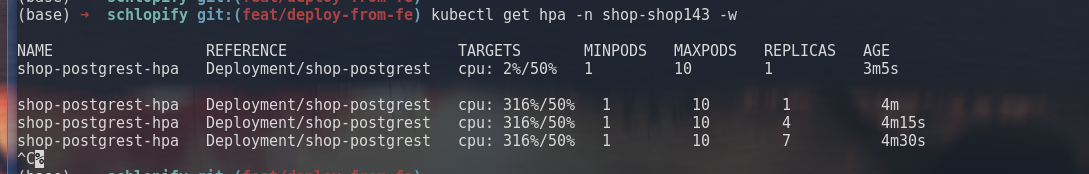
\includegraphics[width=\textwidth]{images/hpa-screenshot.png}
    \caption{Horizontal Pod Autoscaler Scaling PostgREST Pods}
\end{figure}













\newpage
%------------------------------------------------
% SECURITY CONSIDERATIONS
%------------------------------------------------

\chapter{Security Considerations}

Security is an important aspect of cloud-native and multi-tenant applications. Since Schlopify dynamically provisions isolated infrastructures for different tenants, several architectural decisions were made to improve resource isolation and operational security within the Kubernetes environment.

\section{Namespace Isolation}

Each tenant is deployed within a separate Kubernetes namespace. Namespace isolation helps prevent interference between tenant resources and simplifies access management, monitoring, and infrastructure administration.

This approach improves:

\begin{itemize}

    \item Logical separation of tenant workloads
    \item Resource organization
    \item Simplified infrastructure management
    \item Controlled access to tenant-specific services

\end{itemize}

\section{Role-Based Access Control (RBAC)}

Kubernetes Role-Based Access Control (RBAC) policies are used to manage permissions for platform services and provisioning operations. RBAC ensures that services interact only with the resources they are authorized to access.

This helps reduce unnecessary privilege exposure within the Kubernetes cluster.

\section{Containerized Service Isolation}

All application components are deployed as isolated Docker containers. Containerization improves process isolation and minimizes dependency conflicts between services.

Using Kubernetes orchestration further improves security by managing deployments and restricting interactions between workloads.

\section{Ingress and Network Configuration}

Ingress resources are configured to manage external routing for tenant applications. Controlled routing ensures that tenant services remain accessible only through configured endpoints.

The use of Kubernetes networking mechanisms also simplifies service discovery and communication management within the cluster.

\section{Future Security Enhancements}

Although the current implementation focuses primarily on deployment automation and tenant provisioning, several advanced security improvements can be integrated in future versions of the platform.

Planned enhancements include:

\begin{itemize}

    \item HashiCorp Vault integration for secret management
    \item HTTPS and TLS certificate management
    \item Network policies for pod-level communication control
    \item Centralized monitoring and threat detection
    \item Secure CI/CD pipeline integration
    \item Container vulnerability scanning

\end{itemize}













\newpage
%------------------------------------------------
% CHALLENGES FACED
%------------------------------------------------

\chapter{Challenges Faced}

During the development and deployment of Schlopify, several technical and architectural challenges were encountered. Since the project involved Kubernetes orchestration, dynamic infrastructure provisioning, and multi-tenant resource management, significant effort was required to ensure reliable deployment and proper integration between services.

\section{Kubernetes Configuration Complexity}

Managing Kubernetes resources such as deployments, services, ingress configurations, namespaces, and RBAC policies introduced considerable complexity during development. Ensuring proper communication between services and maintaining stable deployments required extensive testing and debugging.

\section{Dynamic Tenant Provisioning}

Implementing automated tenant provisioning using Kubernetes APIs was one of the major challenges in the project. The provisioning logic had to dynamically create namespaces, deploy resources, configure networking, and initialize databases without manual intervention.

Handling failures and maintaining consistency during the provisioning workflow required careful resource management and validation.

\section{Ingress and Networking Issues}

Configuring ingress routing and local DNS resolution using \texttt{nip.io} introduced networking challenges during deployment. Properly exposing tenant-specific services and ensuring correct routing behavior required multiple iterations and testing.

\section{Container and Resource Management}

Managing multiple containerized services for each tenant increased the complexity of deployment and resource allocation. Efficiently organizing services while maintaining tenant isolation required proper namespace management and Kubernetes orchestration.

\section{Autoscaling Configuration}

Configuring Horizontal Pod Autoscaling (HPA) for dynamically provisioned services required understanding Kubernetes scaling policies and workload management. Ensuring that autoscaling worked reliably under different conditions was a significant challenge.

\section{CI/CD and Monitoring Integration}

Integrating Jenkins pipelines with GitHub webhooks, configuring Ansible playbooks for deployment automation, and setting up the ELK Stack for centralized logging required significant effort in pipeline configuration and service coordination across the Kubernetes cluster.














\newpage

%------------------------------------------------
% RESULTS AND OBSERVATIONS
%------------------------------------------------

\chapter{Results and Observations}

The implementation of Schlopify successfully demonstrated the practical application of DevOps methodologies, Kubernetes orchestration, and cloud-native deployment strategies for building a scalable multi-tenant SaaS platform.

\section{Successful Multi-Tenant Deployment}

The platform was able to dynamically provision isolated tenant environments using Kubernetes namespaces. Each tenant received dedicated infrastructure resources including databases, APIs, frontend services, and ingress configurations.

The automated provisioning workflow significantly reduced manual deployment effort and improved infrastructure consistency.

\section{Containerized Microservices Architecture}

All major platform components were successfully containerized using Docker and deployed within Kubernetes clusters. The microservices-based design improved modularity, scalability, and maintainability of the platform.

The architecture enabled independent deployment and management of:

\begin{itemize}

    \item Frontend applications
    \item Backend APIs
    \item Authentication services
    \item Database services
    \item Tenant-specific APIs

\end{itemize}

\section{Kubernetes-Based Automation}

Kubernetes orchestration successfully managed deployments, networking, ingress routing, and scaling operations. Namespace-based isolation improved tenant management and simplified infrastructure organization.

The use of custom deployment scripts automated image loading and infrastructure setup for local Kubernetes environments such as Minikube and Kind.

\section{Horizontal Pod Autoscaling}

Horizontal Pod Autoscaling (HPA) was successfully integrated for PostgREST services. The autoscaling mechanism dynamically adjusted pod counts based on workload requirements, improving scalability and resource utilization.

\section{Observations}

The project demonstrated that Kubernetes can effectively be used not only for deployment orchestration but also as a dynamic infrastructure provisioning platform for SaaS applications.

The implementation also highlighted the importance of:

\begin{itemize}

    \item Infrastructure automation
    \item Namespace-based isolation
    \item Container orchestration
    \item Modular microservices design
    \item Scalable deployment workflows

\end{itemize}

Jenkins CI/CD pipelines with GitHub webhook triggers, Ansible-based configuration management, and ELK Stack monitoring were also successfully integrated, providing automated deployment workflows and centralized observability across the platform.

\begin{figure}[H]
    \centering
    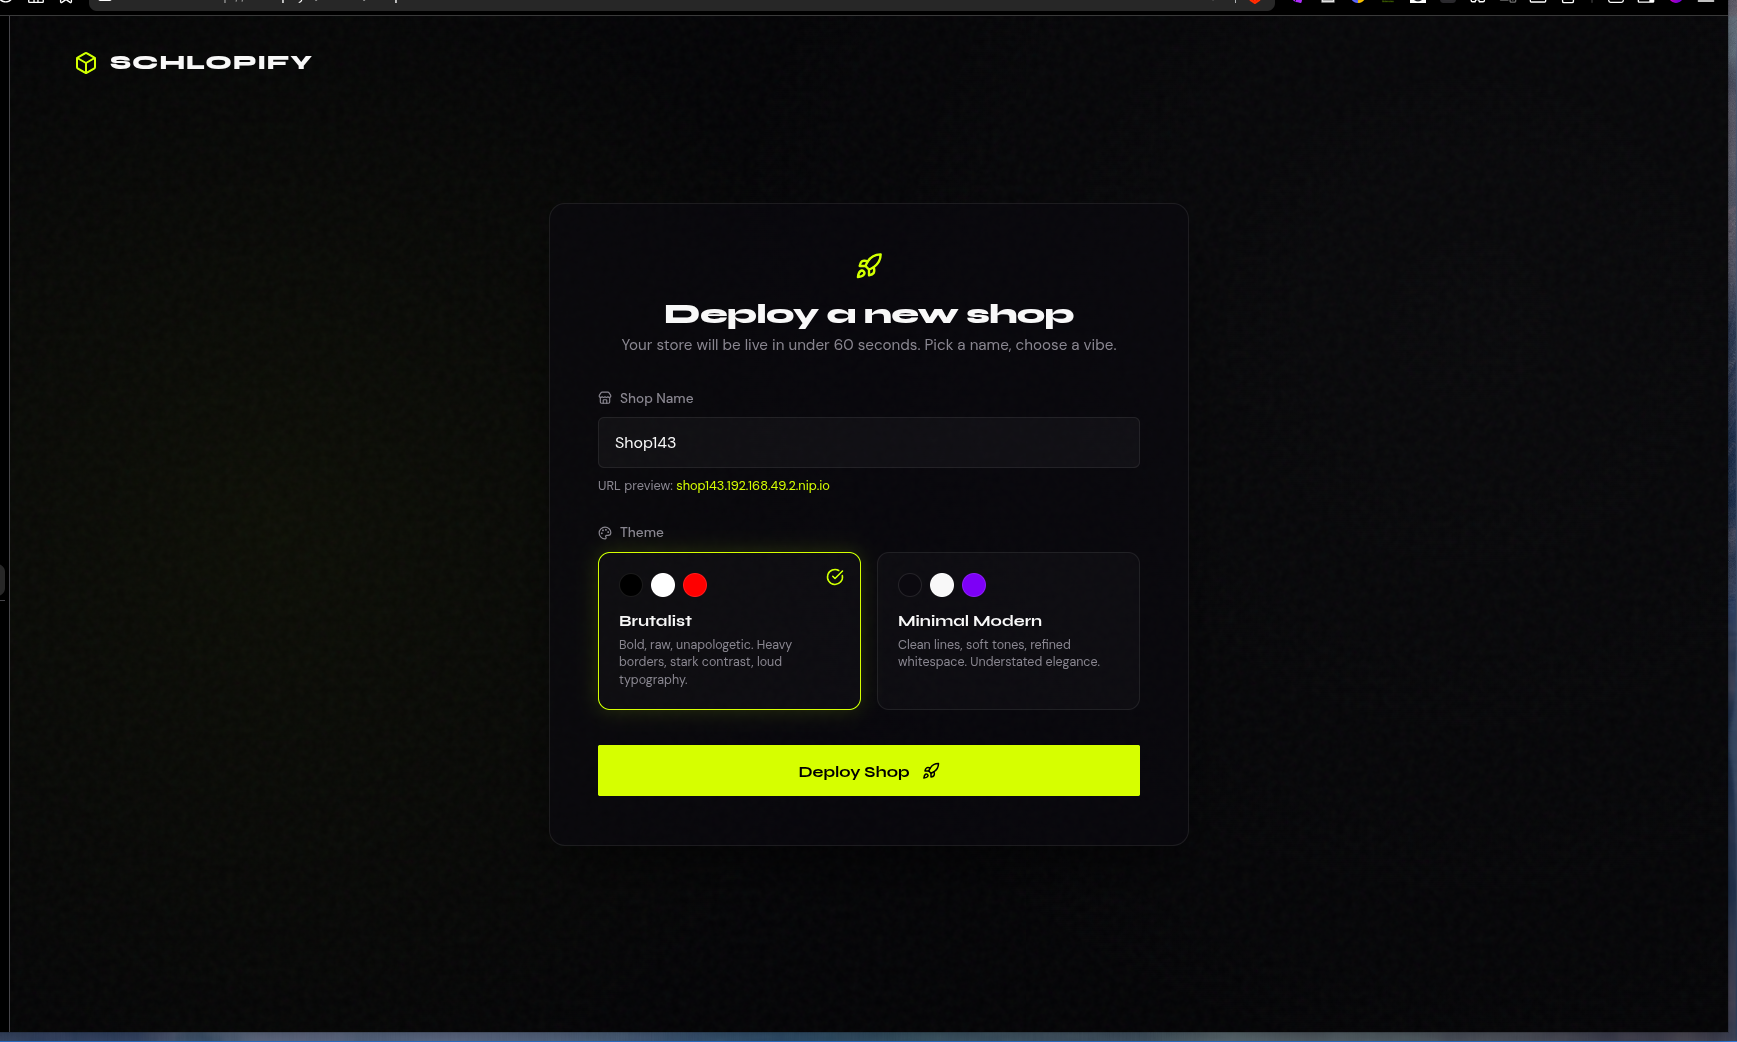
\includegraphics[width=\textwidth]{images/ui-1.png}
    \caption{Shop Deployment Interface}
\end{figure}

\begin{figure}[H]
    \centering
    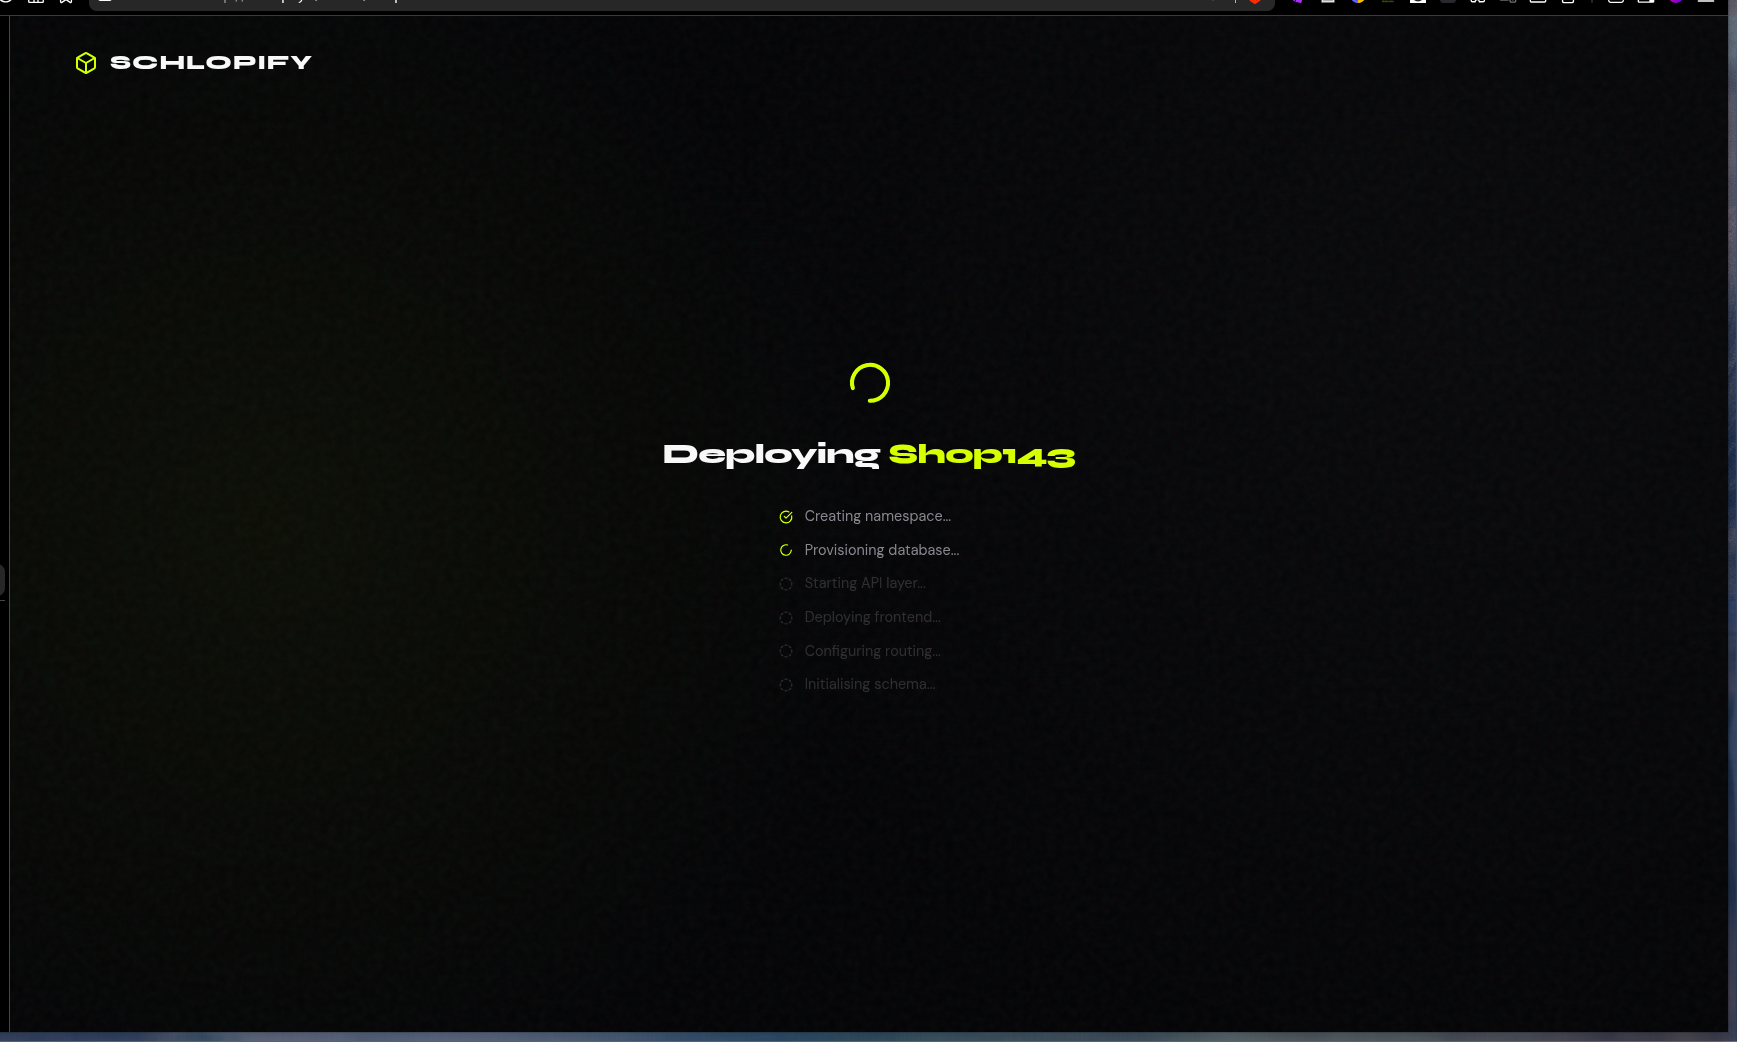
\includegraphics[width=\textwidth]{images/ui-2.png}
    \caption{Shop Deployment Progress}
\end{figure}

\begin{figure}[H]
    \centering
    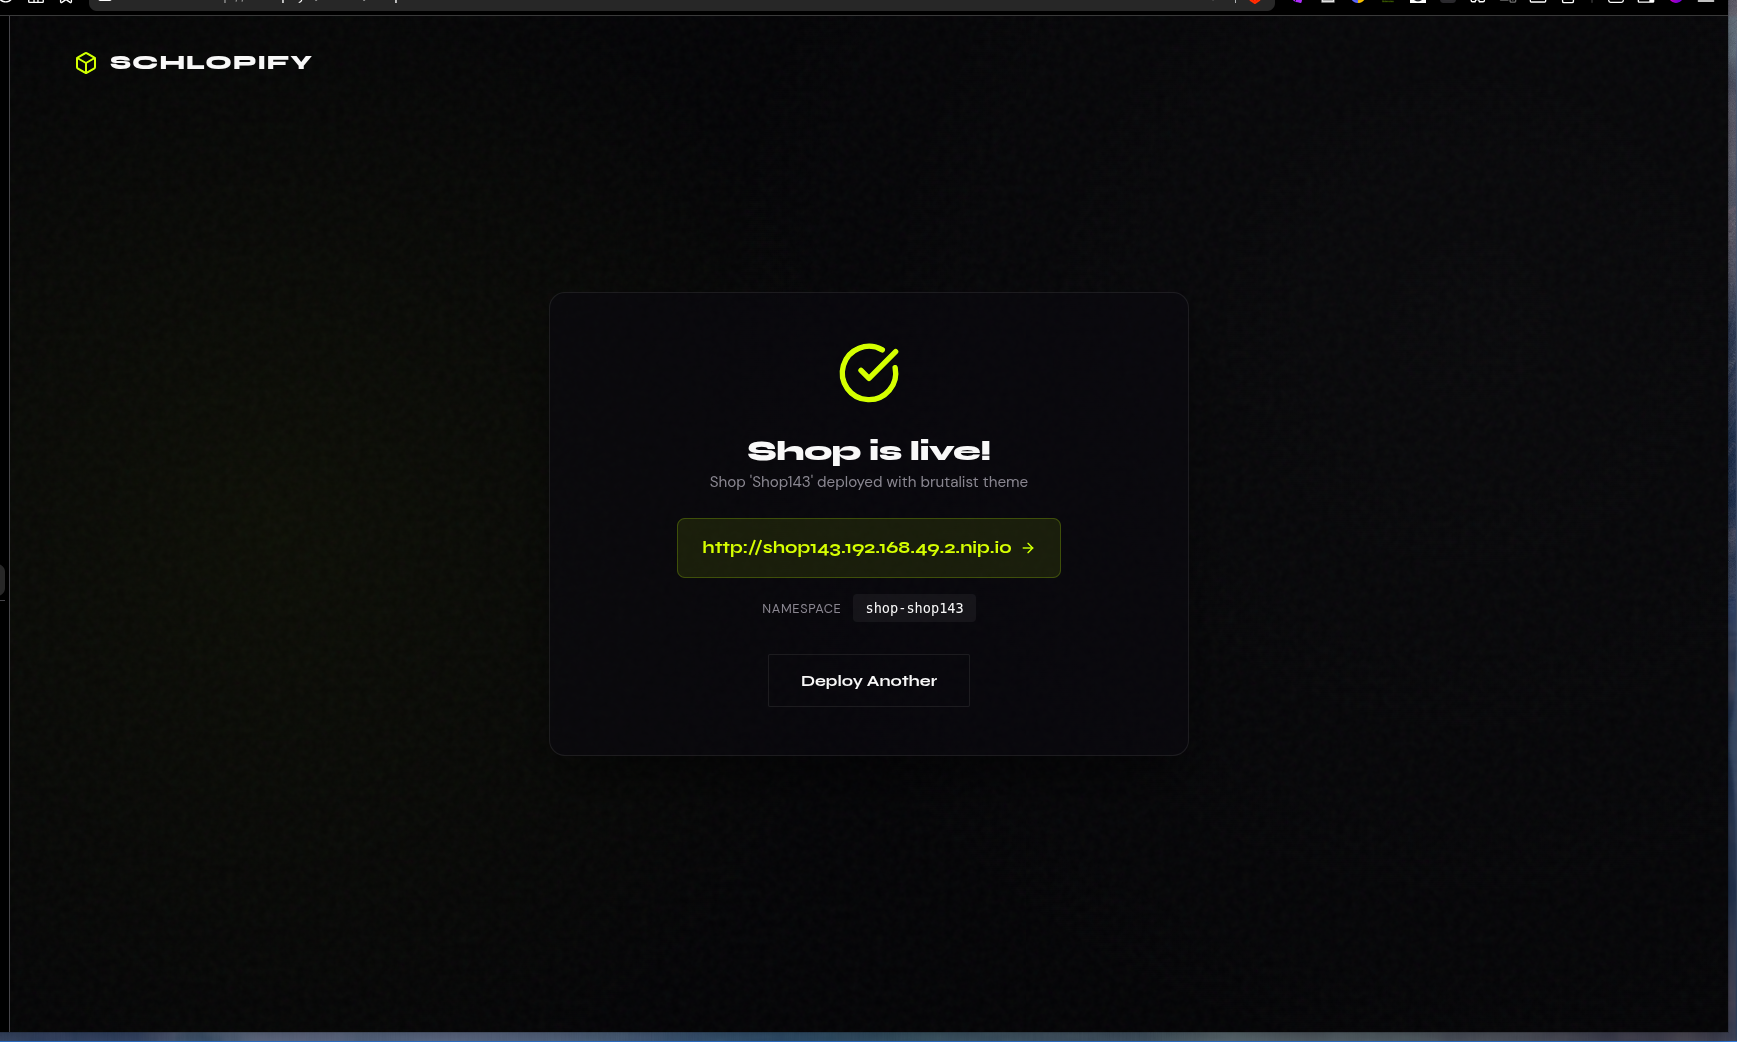
\includegraphics[width=\textwidth]{images/ui-3.png}
    \caption{Successful Tenant Deployment Result}
\end{figure}











\newpage
%------------------------------------------------
% FUTURE ENHANCEMENTS
%------------------------------------------------

\chapter{Future Enhancements}

Schlopify successfully implements dynamic tenant provisioning, Kubernetes-based orchestration, Jenkins CI/CD pipelines, Ansible automation, and ELK Stack monitoring. Several additional features can be added in future versions of the platform to further improve scalability and security.

\section{Advanced Security Features}

Several additional security mechanisms can be implemented to strengthen platform security:

\begin{itemize}

    \item HashiCorp Vault for secret management
    \item HTTPS and TLS certificate automation
    \item Kubernetes Network Policies
    \item Container vulnerability scanning
    \item Secure CI/CD workflows

\end{itemize}

\section{Cloud Deployment Support}

The current platform is designed primarily for local Kubernetes environments such as Minikube and Kind. Future versions can support deployment on cloud platforms including:

\begin{itemize}

    \item Amazon Web Services (AWS)
    \item Google Cloud Platform (GCP)
    \item Microsoft Azure

\end{itemize}

Cloud deployment support would improve scalability, availability, and production readiness.

\section{Enhanced Scalability Features}

Future scalability improvements may include:

\begin{itemize}

    \item Advanced autoscaling policies
    \item Load balancing optimizations
    \item Distributed caching systems
    \item Database replication and backup strategies

\end{itemize}

\section{Production-Grade SaaS Features}

Additional application-level features can also be introduced, such as:

\begin{itemize}

    \item Payment gateway integration
    \item Tenant analytics dashboards
    \item Multi-region deployments
    \item User behavior tracking
    \item Automated backup and recovery systems

\end{itemize}

These enhancements would further improve the platform and make it more suitable for real-world production environments.











\newpage
%------------------------------------------------
% CONCLUSION
%------------------------------------------------

\chapter{Conclusion}

Schlopify successfully demonstrates the practical implementation of modern DevOps methodologies and cloud-native deployment practices for building a scalable multi-tenant e-commerce platform. The project utilizes Docker for containerization and Kubernetes for orchestration, enabling efficient deployment, scaling, and management of microservices-based applications.

One of the major achievements of the platform is the implementation of dynamic tenant provisioning using Kubernetes APIs and Golang. The system is capable of automatically creating isolated tenant infrastructures, including namespaces, databases, APIs, frontend services, ingress configurations, and scaling policies, without requiring manual intervention.

The project also demonstrates the effective use of Kubernetes features such as namespace isolation, ingress routing, RBAC policies, and Horizontal Pod Autoscaling (HPA) for improving scalability and infrastructure management.

The platform also integrates Jenkins CI/CD pipelines with GitHub webhook triggers for automated deployments, Ansible for configuration management, and the ELK Stack for centralized logging and monitoring. Although Vault-based secret management remains a planned enhancement, the current implementation establishes a strong and comprehensive foundation for scalable SaaS infrastructure management.

Overall, the project provided valuable practical experience in containerization, Kubernetes orchestration, infrastructure automation, and cloud-native application deployment. The architecture and implementation of Schlopify reflect real-world DevOps concepts and demonstrate how automated infrastructure provisioning can simplify the deployment and management of multi-tenant platforms.














\newpage
%------------------------------------------------
% REFERENCES
%------------------------------------------------

\chapter{References}

\begin{enumerate}

    \item Kubernetes Documentation. Available at: \\
    \url{https://kubernetes.io/docs/}

    \item Docker Documentation. Available at: \\
    \url{https://docs.docker.com/}

    \item Golang Documentation. Available at: \\
    \url{https://go.dev/doc/}

    \item PostgreSQL Documentation. Available at: \\
    \url{https://www.postgresql.org/docs/}

    \item PostgREST Documentation. Available at: \\
    \url{https://postgrest.org/}

    \item Kubernetes Horizontal Pod Autoscaler Documentation. Available at: \\
    \url{https://kubernetes.io/docs/tasks/run-application/horizontal-pod-autoscale/}

    \item Minikube Documentation. Available at: \\
    \url{https://minikube.sigs.k8s.io/docs/}

    \item Kind Documentation. Available at: \\
    \url{https://kind.sigs.k8s.io/}

    \item HashiCorp Vault Documentation. Available at: \\
    \url{https://developer.hashicorp.com/vault/docs}

    \item Elasticsearch Documentation. Available at: \\
    \url{https://www.elastic.co/docs}

    \item Jenkins Documentation. Available at: \\
    \url{https://www.jenkins.io/doc/}

    \item Schlopify GitHub Repository. Available at: \\
    \url{https://github.com/shreyasg-git/schlopify}

\end{enumerate}



\end{document}
